

\section{Proposed method}

\subsection{Graph construction} 


Autism spectrum disorder (ASD) is now recognized to occur in more than 1\% of children. Despite continuing research advances, their pace and clinical impact have not kept up with the urgency to identify ways of determining the diagnosis at earlier ages, selecting optimal treatments, and predicting outcomes. The researchers \cite{Parisot17} proposed to tackle those challenges and applied their method on the Autism Brain Imaging Data Exchange (ABIDE) dataset, which consists of highly heterogeneous functional MRI data acquired at multiple sites. Resting-state functional magnetic resonance imaging (rs-fMRI) is a neuroimaging technique that measures and analyzes brain activity in a resting state, i.e., when a person is not engaged in any specific task. 
It is based on the principle that different regions of the brain exhibit correlated spontaneous fluctuations in blood oxygen level-dependent (BOLD) signals even in the absence of an explicit stimulus or task. These fluctuations are thought to reflect the intrinsic functional connectivity of the brain. 

The authors \cite{Parisot17} proposed to construct a population graph integrating imaging and non-imaging data. 
They defined the feature vector $x(v)$ of each patient $v$ as the vectorized form $X_{v}$ of its functional connectivity matrix. Connectivity matrices represent the strength of functional connections between different brain regions for a given subject. They are derived from rs-fMRI data by computing the Pearson's correlation coefficient between brain regions' activity patterns, offering a concise representation of interregional communication within brain regions. \blue{Note that they also applied the Fisher transform of the Pearson correlation but we did not do it}. Given the matrix's high dimensionality (6700 \blue{review true number}), they employed a ridge classifier to pinpoint the most discriminative features within the training set. 

They modeled the interactions between individuals via the definition of the graph edges $\EE$ which writes as follows for two nodes $v$ and $v'$ :
$$ 
    \WW(v, v') = Sim(X_v, X_{v'}) \left[\delta_{M_{SEX}(v)}(M_{SEX}(v')) + \delta_{M_{SITE}(v)}(M_{SITE}(v')) \right]
$$

$\delta$ is the Kronecker delta function.  $M_{SITE}$ and $M_{SEX}$ are contextual information. $Sim$ is a similarity measures between the connectivity matrices of the subjects $v$ and $v'$. In \cite{Parisot17}, the authors used the correlation distance 
$$
Sim(X_v, X_{v'}) =  1 - \frac{(X_v - \bar{X}_v).(X_{v'} - \bar{X}_{v'})}{\norm{X_v -\bar{X}_{v}}_2\norm{X_{v'} - \bar{X}_{v'}}_2}
$$
where $\bar{X}_v$ is the mean of the elements of the vectorized connectivity matrix of patient $v$. 

On the figure \ref{fig:sorted_adjacency}, certain sets or squares stand out with significantly higher correlation along the diagonal exhibiting the proximity between those metadata information. 

\begin{figure}[h!]
    \centering
    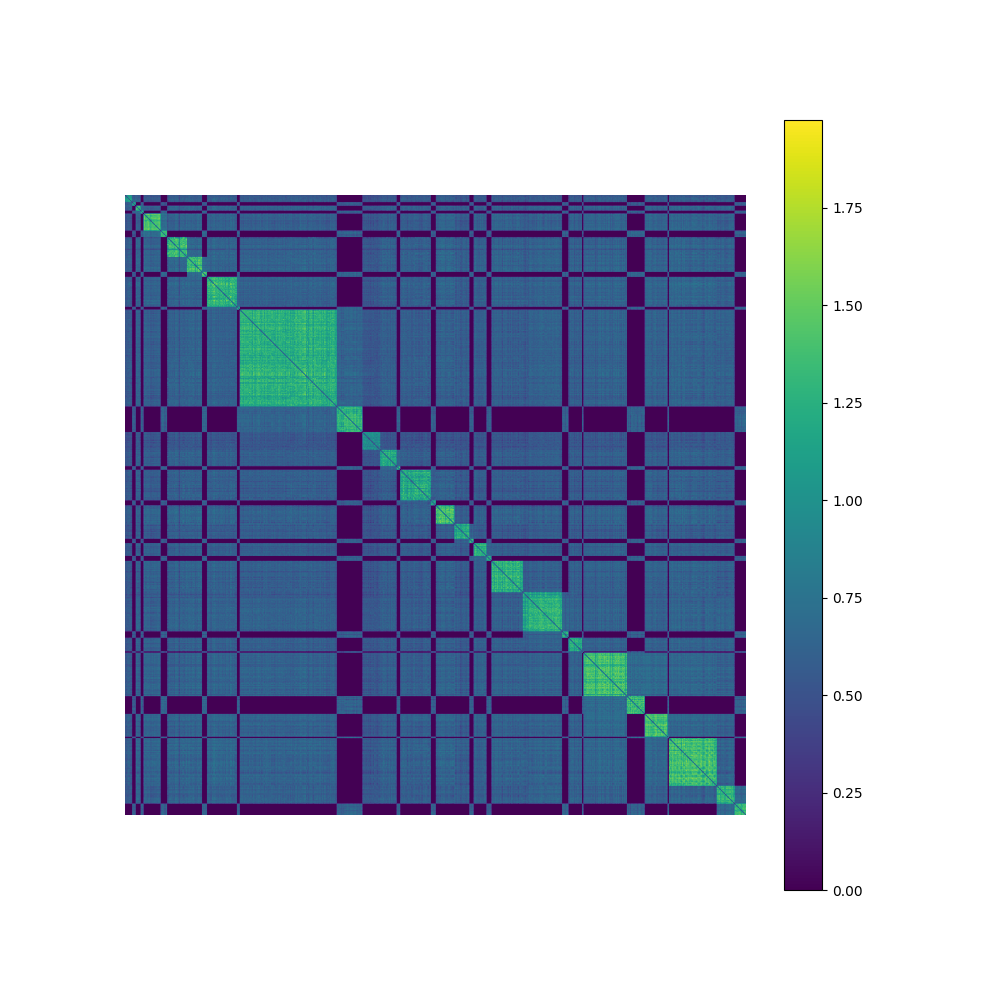
\includegraphics[width=0.45\textwidth]{figures/sorted_adjacency_by_site_id_by_sex.png}
    \caption{Edge weights sorted by acquisation sites and sex.}
    \Description{}
    \label{fig:sorted_adjacency}
\end{figure}

To classify from this brain population graph, the authors \cite{Parisot17} proposed to use a convolutional neural network (CNN) on graphs. We will now present the mathematical framework of graph convolutional neural networks.

\subsection{Mathematical framework on Graph Spectral Theory}
\subsubsection{The main challenges of signal processing on graphs} 

Graphs are widely used thanks to their generic data representation forms which are useful for describing the geometric structures of data domains in very different application fields, including social, energy, transportation, and brain modelisation.
However, classical tools and techniques from signal processing can not be used seamlessly on graphs unlike audio signal and images \cite{shuman_emerging_2013}.

In particular, graphs have no inherent ordering of the vertices, unlike images where pixel is uniquely identified by its position within the image. We therefore need algorithms that are node-order equivariant: they should not depend on the ordering of the nodes \cite{daigavane_understanding_2021}. We may also need localized transforms that compute information about the data at each vertex by using data from a small neighbourhood of vertices close to it in the graph.

Graphs can also be very large but, in our study, we consider sparse population graphs, \ie individuals or nodes are connected to a limited number of nodes \footnote{We also say that the number of edges is linear in the number of nodes.}.
Spectral graph theory has enabled constructing, analyzing, and manipulating graphs.

%In signal processing on graphs, it is leveraged as a tool to define frequency spectra and expansion bases for graph Fourier transforms.

In this section, we present some basic definitions from spectral graph theory that will be needed to apply neural networks on graphs. As stated previously, we consider an undirected, connected, weighted graph $\mathcal{G} = \{\mathcal{V}, \EE, \WW\}$. 

\subsubsection{The non-normalized and normalized Graph Laplacian}

The non-normalized graph Laplacian, also called the combinatorial graph Laplacian, is defined 
as $\mathbf{L} = \mathbf{D}-\mathbf{W}$, where the degree matrix $\mathbf{D}$ 
is a diagonal matrix 
whose $i$th diagonal element, $d_i$, is equal to the sum of the weights of all edges incident to vertex $i$
(e.g. the sum over the rows of $\WW$).
%The graph Laplacian is a difference operator defined for any signal $f$, as follows :
%$$
%(\mathbf{L}f)(i) = \sum_{j\in\mathcal{N}_i} W_{i, j}[f(i) - f(j)]
%$$
%where $\mathcal{N}_i$ is the set of vertices connected to vertex $i$ by an edge.

The graph Laplacian $\mathbf{L}$ is a real symmetric matrix, it has therefore real, non-negative eigenvalues $\{\lambda_l\}_{l=0, \dots, N-1}$. 
We denote their associated  orthonormal eigenvectors by $\{u_l\}_{l=0,\dots, N-1}$. In the following, $\Lambda$ and $U$ denote the diagonal matrix of eigenvalues and the matrix of eigenvectors, respectively.

Since we consider connected graphs, the eigenvalue $\lambda_0=0$ has multiplicity $1$  \cite{shuman_emerging_2013}. 
\textit{(There are as many null eigen values as there are connected components in the graph.)}

A popular practice is to normalize each weight $W_{i, j}$ by a factor of $\frac{1}{\sqrt{d_id_j}}$.
Doing so leads to the normalized graph Laplacian, which is defined as $\widetilde{\mathbf{L}} = D^{-1/2}\mathbf{L}D^{-1/2} = I_N - D^{-1/2}\mathbf{W}D^{-1/2}$. This strategy is used to improve the stability of gradient flow during backpropagation in neural networks. This can be valuable in mitigating the vanishing gradient problem and facilitating the training of deeper and more expressive models on graph data.


\subsubsection{A Graph Fourier Transform and Notion of Frequency}
The Fourier transform for analogous function $f$
$$
\hat{f}(\xi) = \sca{f}{e^{2\pi i\xi t}} = \int_{\RR} f(t)e^{-2\pi i \xi t}dt
$$
is the expansion of a function $f$ in terms of the complex exponentials, which are the eigenfunctions of the one-dimensional Laplace operator $\Delta$ :
$$
-\Delta (e^{2\pi i \xi t}) = -\frac{\partial^2}{\partial t^2} e^{2\pi i \xi t} = (2\pi i\xi)^2 e^{2\pi i \xi t}
$$
Similarly, we can define the \textit{Graph Fourier Transform} $\hat{f}$ of any function on the vertices of $\GG$ as the expansion of $f$ in terms of the eigenvectors of the graph Laplacian $\hat{f}(\lambda_l) = \sca{f}{u_l} = \sum_{i=1}^{N} f(i)u_l^*(i)$ : 
where $u_l^*(i)$ is the conjugate of $u_l(i)$ : 
\begin{equation}
    \hat{f} = U^Tf
\end{equation}

The \textit{inverse graph Fourier transform} is then given by $f(i) = \sum_{i=1}^{N} \hat{f}(\lambda_i)u_l(i)$ : 
\begin{equation}
    f = U\hat{f}
\end{equation}

Note that, in our case, the signal is $f:\mathcal{V}\rightarrow\RR^N$ that associate a feature vector to each node of the graph.

\subsubsection{Spectral Graph Convolutions}

Spectral convolution of the signal $f$ with a filter $g_\theta$ is defined as $g_\theta * f = g_\theta(\widetilde{\mathbf{L}})f = Ug_\theta(\Lambda)U^Tf = U g_\theta(\Lambda)\hat{f}$. 
Indeed, we recover the property that the convolution in the vertex domain is equivalent to a multiplication in the graph spectral domain.

Polynomial filters, defined as $g_\theta(\Lambda) = \sum_{k=0}^{K-1}\theta_k\Lambda^k$, are commonly used in localized convolutions. Those filters are localized thanks to the lemma 5.2 in \cite{hammond_wavelets_2011}. We can show that for some integer $s$ and for any 
vertices $m$ and $n$ in the graph $\GG$, if $d_\GG(m, n) > s$ then $(L^s)_{m, n} = 0$. $d_\GG(m, n)$ denotes the number of edges in the shortest path connecting the nodes $m$ and $n$.
It follows that a $K$-order polynomial filter is strictly $K$-localized, \ie it only depends on the $K$-hop neighbourhood of each vertex. In the studied paper \cite{Parisot17}, the authors chose $K=3$.\\ 
Futhermore, according to the lemma \ref{lemma:chebyDecomposition}, such filters can be well approximated by a truncated Chebyshev expansion of the form $g_\theta(\widetilde{\mathbf{L}}) = \sum_{k=0}^{K-1}\theta_kT_k(\widetilde{\mathbf{L}})$ where $T_k$ is the $k$th Chebyshev polynomial of the first kind.
\begin{lemma}\label{lemma:chebyDecomposition}
    In the appropriate Sobolev space, the set of Chebyshev polynomials form an orthonormal basis, so that a function in the same space can, on $-1\leq x \leq 1$, be expressed via the expansion : $$g(x) = \sum_{n=0}^{\infty} a_nT_n(x)$$.
\end{lemma}
This decomposition significantly reduces the computational complexity of the convolution operator \cite{Parisot17}.

%polynomials of Laplacian of degree $d$ : the node $v$ is convolved with nodes that are at most at a distance $d$. Thus, these polynomials filters are localized.

\subsubsection{A simple illustration}

We have implemented a simple application of the spectral graph convolution on a toy graph. 
On the illustration \ref{fig:toyGraph}, we notice that the greater the order of the convolution,  the more the signal is smoothed, and the less the graph laplacian have null coefficients.

 \begin{figure}
    \centering
    \begin{subfigure}{0.45\textwidth}
        \centering
        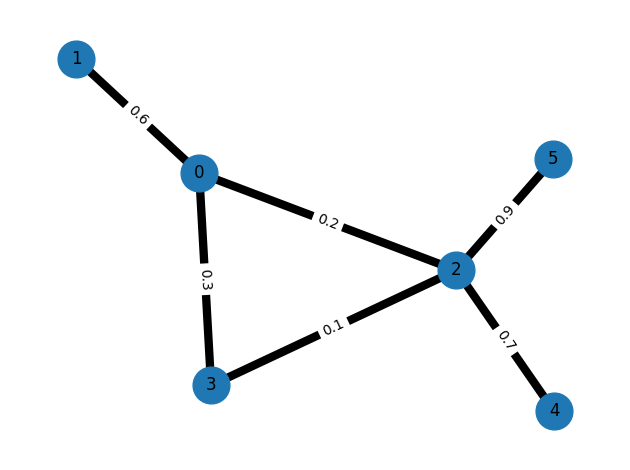
\includegraphics[width=0.45\textwidth]{figures/toy_graph_init.png}
        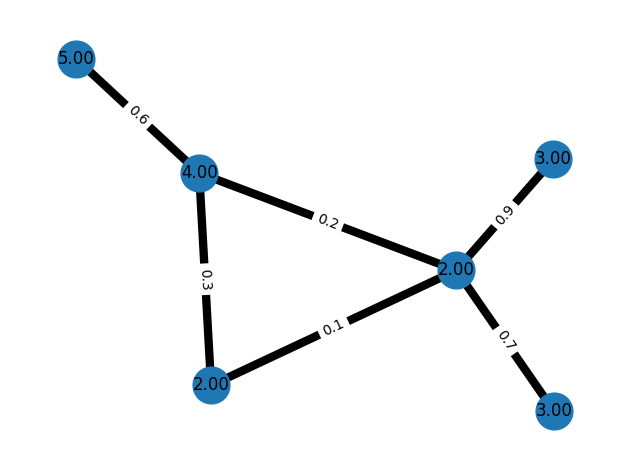
\includegraphics[width=0.45\textwidth]{figures/toy_graph_conv_K1.png}
        \caption{Toy graph\\ $\leftarrow$ indexes of the nodes | initial features values ($K=1$) $\rightarrow$}
    \end{subfigure}
    \hfill
    \begin{subfigure}{0.45\textwidth}
        \centering
        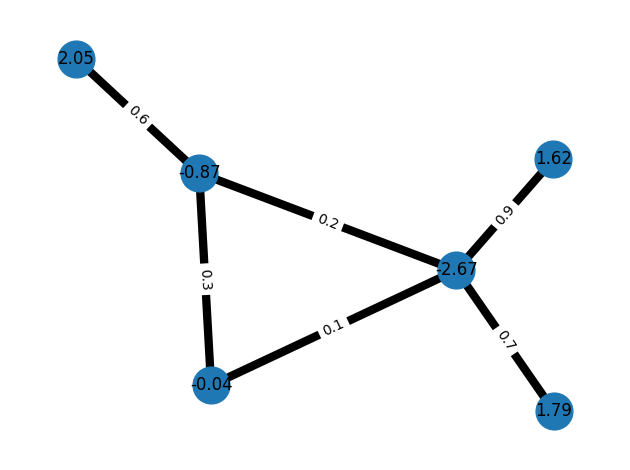
\includegraphics[width=0.45\textwidth]{figures/toy_graph_conv_K2.png}
        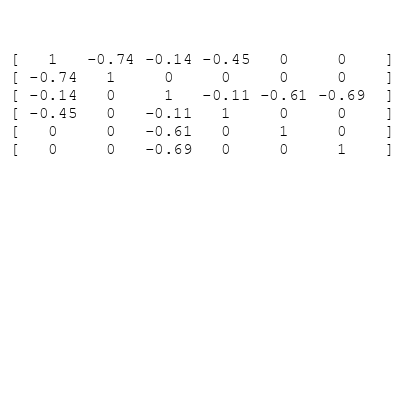
\includegraphics[width=0.45\textwidth]{figures/lap1.png}
        \caption{$\leftarrow$ After convolution with $K=2$ | $\tilde{L}$ $\rightarrow$}
    \end{subfigure}
    \hfill
    \begin{subfigure}{0.45\textwidth}
        \centering
        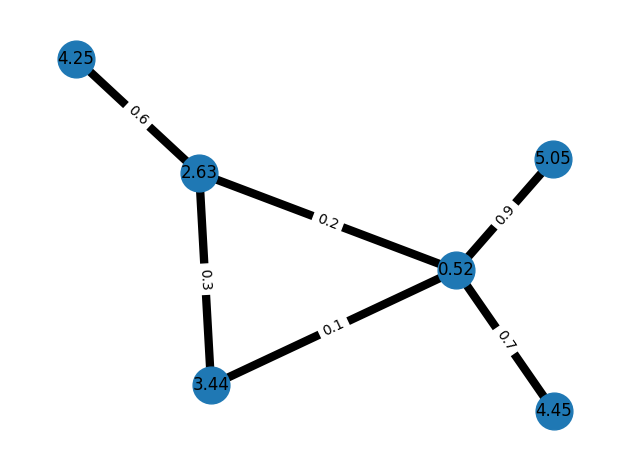
\includegraphics[width=0.45\textwidth]{figures/toy_graph_conv_K3.png}
        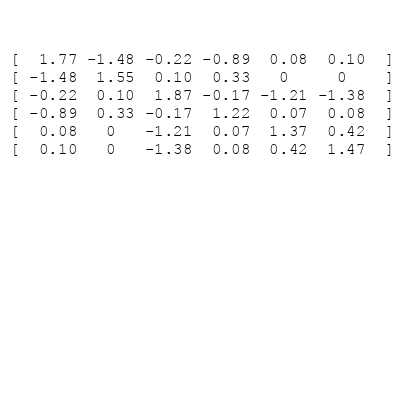
\includegraphics[width=0.45\textwidth]{figures/lap2.png}
        \caption{Convolution with $K=3$ | $\tilde{L}^2$ $\rightarrow$ }
    \end{subfigure}
    \caption{Convolution of a toy graph and the normalized laplacian matrix $\widetilde{\mathbf{L}}^K$ for $K=1, 2, 3$.}
    \label{fig:toyGraph}
    \Description[]{illustration of convolution on graph}
 \end{figure}
For the example displayed in figure \ref{fig:toyGraph}, we initialized the weight of the convolution to one.

